\documentclass[utf8, xcolor=dvipsnames]{beamer}

%\usepackage{default}
%\usepackage{beamerthemesplit}
%\usepackage{beamerthemeAnnArbor}
% \usepackage{beamerthemeAntibes}
% \usepackage{beamerthemeBergen}
% \usepackage{beamerthemeBerkeley}
% \usepackage{beamerthemeBerlin}
% \usepackage{beamerthemeBoadilla}
% \usepackage{beamerthemeboxes}
% \usepackage{beamerthemeCambridgeUS}
% \usepackage{beamerthemeCopenhagen}
% \usepackage{beamerthemeDarmstadt}
% \usepackage{beamerthemedefault}
% \usepackage{beamerthemeDresden}
% \usepackage{beamerthemeFrankfurt}
% \usepackage{beamerthemeGoettingen}
% \usepackage{beamerthemeHannover}
% \usepackage{beamerthemeIlmenau}
% \usepackage{beamerthemeJuanLesPins}
% \usepackage{beamerthemeLuebeck}
% \usepackage{beamerthemeMadrid}
% \usepackage{beamerthemeMalmoe}
% \usepackage{beamerthemeMarburg}
% \usepackage{beamerthemeMontpellier}
% \usepackage{beamerthemePaloAlto}
% \usepackage{beamerthemePittsburgh}
% \usepackage{beamerthemeRochester}
% \usepackage{beamerthemeSingapore}
% \usepackage{beamerthemeSzeged}
% \usepackage{beamerthemeWarsaw}
\usepackage{beamerthemeFreiburg}

% Color scheme blau oder anders?
\usecolortheme[named=Blue]{structure}
% \usecolortheme{wolverine}
\setbeamercolor{block title}{fg=craneblue,bg=craneorange}

% Mit oder ohne Schatten?
\setbeamertemplate{blocks}[rounded][shadow=false]

%\usepackage{pstricks}
\usepackage{german}
\usepackage{ragged2e}

%% zum Drucken:
% \usepackage{pgfpages}
% \pgfpagesuselayout{resize to}[a4paper,border shrink=5mm,landscape]
% \pgfpagesuselayout{2 on 1}[a4paper,border shrink=5mm]
% \pgfpagesuselayout{4 on 1}[a4paper,border shrink=5mm,landscape]
% \pgfpagesuselayout{8 on 1}[a4paper,border shrink=5mm]
% \pgfpagesuselayout{16 on 1}[a4paper,border shrink=5mm,landscape]
\renewcommand{\t}[1]{\texttt{#1}}


\title[Ethersex]{Das Ethersex-Projekt}
\subtitle{Einführung}
\author[]{stesie \and stettberger\newline \texttt{ethersex-devel@list.zerties.org}}
\date[EaHegg 10]{Easterhegg 2010}

\titlegraphic{
\includegraphics[width=1.5cm]{gnu-fdl.png}}
\logo{
\includegraphics[width=1.5cm]{./bunnies-bg.png}}

\begin{document}

\frame{
  \frametitle{Ethersex}
  \titlepage
}

\frame{
  \frametitle{Übersicht}
  \tableofcontents
}

%% \frame{
%%   \begin{block}<1->{Zitat}
%%     \begin{quote}
%%       \justifying{
%% 	Der Urquell aller technischen Errungenschaften
%% 	ist die göttliche Neugier und der Spieltrieb des bastelnden und grübelnden Forschers
%% 	und nicht minder die konstruktive Fantasie des technischen Erfinders...\\
%% 	(A. Einstein: Eröffnung IFA 1930)
%%       }
%%     \end{quote}
%%   \end{block}
%%   \begin{block}<2->{Zusatz}
%%     \begin{quote}
%%       \justifying{
%% 	... und Softwareentwicklers.
%%       }
%%     \end{quote}
%%   \end{block}
%% }

% Vortrag in 3 Teilen: Über Ethersex, Ethersex benutzen, Für Ethersex entwickeln

% Historie, Überblick (Kenndaten, Was macht das Projekt besonders), Abstraktionen (IO, Metaschicht, Kommunikation[ECMD]), 

% Einleitung
\section{Überblick}
\frame{
  \frametitle{Überblick}
  \begin{block}{Mission Target}
    Universelle Plattform für Kommunikation auf Mikrocontrollern
  \end{block}

  \begin{itemize}
    \item Zielplattform: Atmel AVR 8-Bit Mikrocontroller
    \item alternativ für's Debugging nativ unter Linux
    \item Quellcode in C, ergänzt durch Präprozessor m4 
    \item GPLv3 lizenziert (Teile LGPL \& BSD 3-clause)
    \item Dateien: $>1000$ \footnote{Ermittelt mit: find . -type f $\mid$ grep -v git $\mid$ wc -l}
    \item Lines of Code: $\sim73832$ \footnote{Ermittelt mit: find . -name ``*.[hc]'' $\mid$ xargs cat $\mid$ wc -l} zzgl. $\sim6582$ Zeilen m4
    \item Modularer Aufbau: 93 Module $\Rightarrow$ schnell erweiterbar
    \item Gut dokumentiert (fast 100 Seiten Doku, Beispiele)
      % Habe hier die Wiki Seiten mit ethersex Kategorie gezählt (waren 93)

  \end{itemize}
  
}

\begin{frame}
  \begin{center}
    
\includegraphics[width=6cm]{oreally.png}      
  \end{center}
\end{frame}


\subsection{Zielplattform}
\frame{
  \frametitle{-v Zielplatform}
  \begin{itemize}
    \item Programmspeicher (Flash): 8kB - 64kB
    \item RAM: 1 kB - 4 kB 
    \item Kosten pro Chip: 1 EUR - 10 EUR
    \item Auswahl der Hardware über Menuconfig 
    \item Fast alle Module auf allen Prozessoren verfügbar
  \end{itemize}
}

\begin{frame}
  \frametitle{Etherrape}
  \begin{center}
    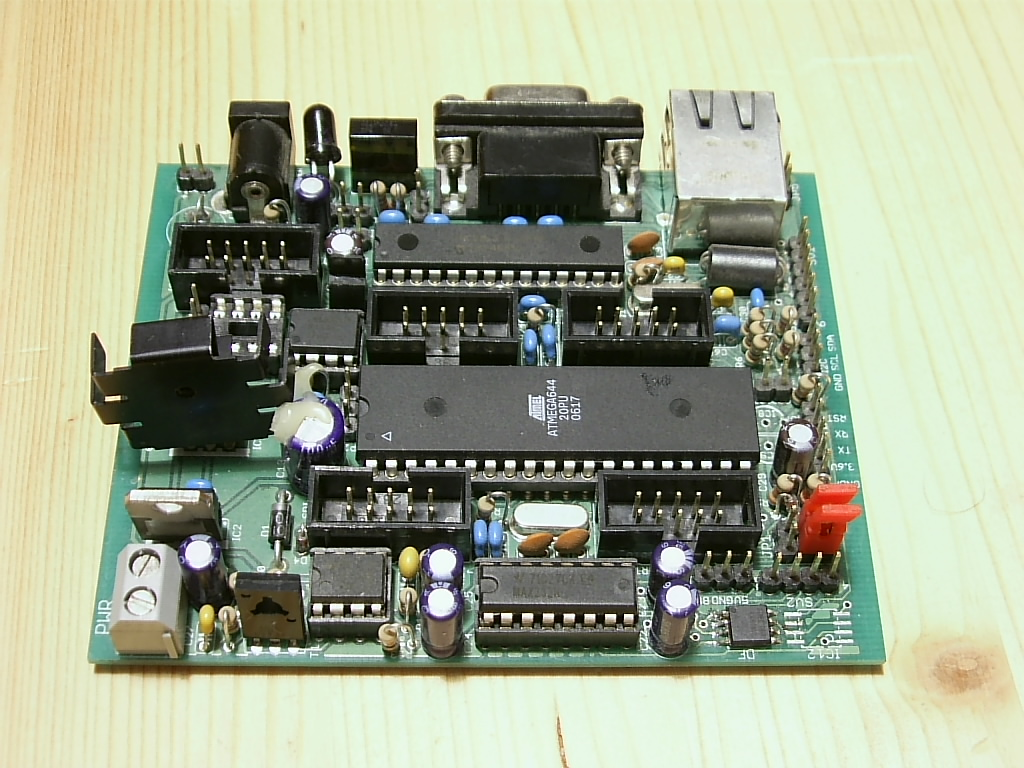
\includegraphics[width=9cm]{Etherrape.jpg}      
  \end{center}
\end{frame}

\begin{frame}
  \frametitle{AVR NetIO - Pollin}
  \begin{center}
    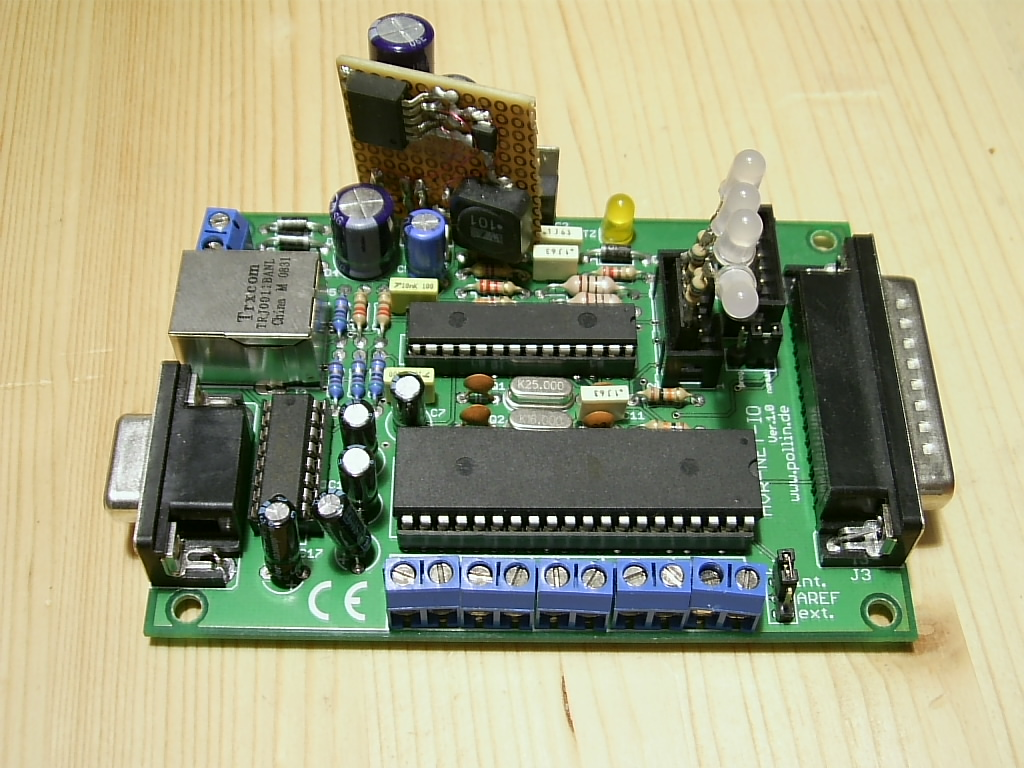
\includegraphics[width=9cm]{Avr-net-io.jpg}      
  \end{center}
\end{frame}

\begin{frame}
  \frametitle{Powerswitch - Eigenbau}
  \begin{center}
    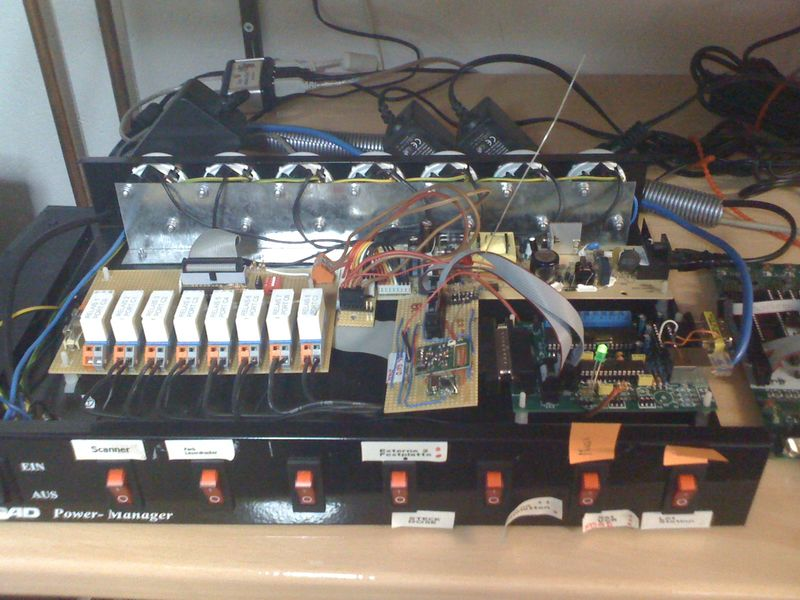
\includegraphics[width=9cm]{Ethersex-Avrnet-GPA.jpg}      
  \end{center}
\end{frame}

\begin{frame}
  \frametitle{PoPuSt - Popellige Pumpensteuerung}
  \begin{center}
    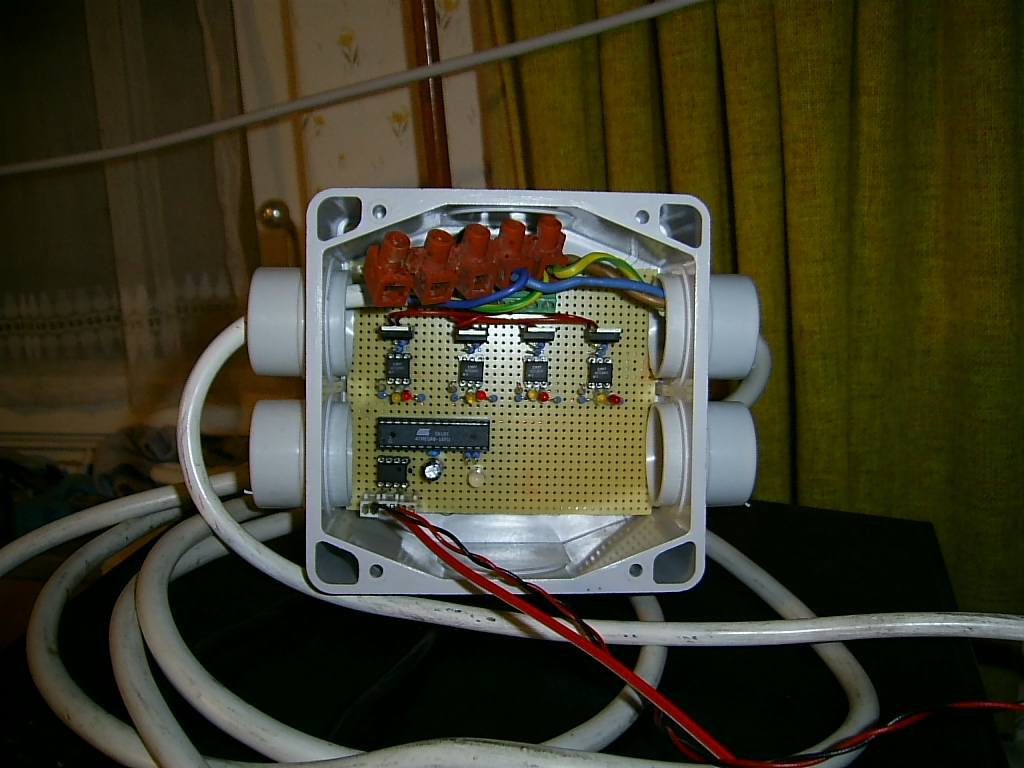
\includegraphics[width=9cm]{TikiImage350.jpg}      
  \end{center}
\end{frame}


\subsection{Kernkonzepte}
\begin{frame}
  \frametitle{Kernkonzepte}
  \begin{itemize}
    \item everything IP
    \item ECMD als einheitliche Interaktionsschnittstelle
    \item Hohe Abstraktion zur Compilezeit
    \item m4, sed, awk and others rule ...
      \pause
    \item ... zur großen Freude unserer Windows-User :-)
  \end{itemize}
\end{frame}

\section{Historie}
\frame{
  \frametitle{Die Entstehungsgeschichte}
  \begin{itemize}
  \item August 06: fd0 startet Etherrape für u23
  \item Dezember 06: fd0's Vortrag am 23C3
  \item August 07: stesie implementiert IPv6, Ethersex wird geforked
  \item Oktober 07: IP über RFM12 wird implementiert, weitere Netzwerkinterfaces folgen
  \item November 07: OpenVPN mit symmetrischer Krypto
  \item Dezember 07: erstes m4 Zeugs
  \item März 08: IP-Router
  \item April 09: Meta-System \& Wechsel zur GPLv3
  \item bis heute: wöchentlich neue Module ...
  \end{itemize}
}

\section{Ethersex Core}
\subsection{Hardware Abstraktion}
\frame{
  \frametitle{Kerntech$\wedge$WBUZZWORD}
  \begin{block}{Menuconfig}
    \begin{itemize}
      \item Konfiguration mit Modulabhänigkeiten
      \item Übernommen vom Linuxkernel
      \item ncurses Interface (DEMO!)
    \end{itemize}
  \end{block}

  \begin{block}{Ethersex META}
    \begin{itemize}
      \item Einzelnes Modul (Ordner) beinhaltet alles Notwendige
      \item Sektion in der .c - Datei
      \item Bsp. \texttt{periodic(meine\_periodic\_func, 50)}
      \item Funktion \t{meine\_periodic\_func} wird jede Sekunde (50 * 20ms) \
        aufgerufen
      \item sed ... $\mid$ m4 ... $>$ meta.c
    \end{itemize}
  \end{block}
  
}
\frame{
  \frametitle{abstract, meta, voodoo ...}
  \begin{block}{Pinning}
    \begin{itemize}
      \item Ordnet Pins einen Namen zu und ermöglicht Zugriff
      \item \t{PIN(RED\_BUTTON, PB1)} - Definition eines Pins
      \item \t{PIN\_SET(RED\_BUTTON)} - Pin auf 5V setzen
      \item Einfaches Verlegen von Anschlüssen
      \item M4 powered        
    \end{itemize}
  \end{block}
  
  \begin{block}{USART}
    \begin{itemize}
    \item Auswahl serieller Schnittstelle via Menuconfig
    \item workarounds für AVR libc Inkonsistenzen
    \item \texttt{usart(UCSR,B) $\mid$= \_BV(usart(TXCIE));}
    \end{itemize}
  \end{block}
}

\subsection{ECMD}
\frame{
  \frametitle{ECMD - Ethersex Command}
  \begin{itemize}
  \item ECMD als zentrale Interaktionsschnittstelle
  \item Einzeilige ASCII Kommandos, ähnlich Shell, batchbar
  \item Bsp.: \t{io get pin 0}
  \item Holt den Eingangsstatus für Port 0 \\
    (PORTA oder PORTB je nach Prozessor)
  \end{itemize}
}

\frame{
  \frametitle{Steuerungsprotokoll ECMD}
  Zugriff auf die ECMD Schnittstelle über: 
  \begin{itemize}
  \item Per Netzwerk 
	\begin{itemize}
	\item TCP (HTTP Protokoll)
	\item TCP
	\item UDP
    \item Jabber
    \item IRC
    \item HTTP ( + Javascript = Dynamische Webseiten)
    \end{itemize} 
  \item Per USB 
  \item Per I2C 
  \item Per RS232/RS485 
  \item $\cdots$
  \end{itemize}
}


\subsection{Control6}
\begin{frame}
  \frametitle{Control6}

  \begin{itemize}
  \item Skriptsprache, basierend auf proto threads
  \item m4 \$foo $<$ control6.src $\mid$ gcc
  \end{itemize}

  \t{\ \ \ THREAD(logging)}\\
  \t{\ \ \ \ \ \ static counter = 0;}\\
  \t{\ \ \ \ \ \ VFS\_LOG(''log'', ''data: \%d{\textbackslash}n'', counter++;}\\
  \t{\ \ \ \ \ \ WAIT(5);}\\
  \t{\ \ \ THREAD\_END(logging)}\\
  \t{}\\
  \t{\ \ \ ON STARTUP DO}\\
  \t{\ \ \ \ \ \ THREAD\_START(logging);}\\
  \t{\ \ \ END}\\
  
  
  \begin{itemize}
  \item m4, m4, m4 ...
  \end{itemize}
\end{frame}

\subsection{Virtual Filesystem}
\frame{
  \frametitle{Virtual File System}
  \begin{itemize}
    \item Verschiedene Backends (SD Karte, Interner Flash, Externer Dataflash)
    \item *nix like interface
    \item \t{vfs\_file\_handle\_t fd = vfs\_open(``log'');}\\
      \t{vfs\_fseek(fd, 23, SEEK\_CUR);}\\
      \t{vfs\_read(fd, buf, 42);}\\
      \t{vfs\_close(fd);}
  \end{itemize}
}

\section{uIP-Stack}
\begin{frame}
  \frametitle{Everything IP - uIP}
  
  \begin{block}{Einschränkungen}
    
    \begin{itemize}
    \item TCP Retransmits
    \item IP Packet Reassembly
    \item Out-Of-Order Reception
    \item Begrenzte Anzahl Connections
    \end{itemize}

  \end{block}

  
  \begin{block}{solutions}
    
    \begin{itemize}
    \item Kodiere Verbindungsstatus
    \item Kein Unterschied zwischen send und retransmit \\
      $\Rightarrow$ Applikation muss Daten reproduzieren können
    \end{itemize}

  \end{block}

\end{frame}


\begin{frame}[fragile]
  \frametitle{Beispiel gefällig?}
  \small{\begin{verbatim}
    void application(void) {
      if(uip_aborted() || uip_closed()) {
        closed();
      }
      if(uip_connected()) {
        connected();
      }
      if(uip_acked()) {
        acked();
      }
      if(uip_newdata()) {
        newdata();
      }
      if(uip_rexmit() || uip_newdata() || uip_acked() 
         || uip_connected() || uip_poll()) {
        senddata();
      }
    }
  \end{verbatim}}

\end{frame}

\subsection{IP Router}
\begin{frame}
  \frametitle{IP Router}
  
  \begin{itemize}
  \item Verschiedene Interfaces: Ethernet, RFM12, ZBus, USB (OpenVPN)
  \item jedes mit eigener IP-Adresse/Mask
  \item Forwarding zwischen Interfaces
  \item ARP-Proxy
  \item IPchair (= Firewalllösung)
  \end{itemize}

\end{frame}


\begin{frame}
  
  \begin{center}
    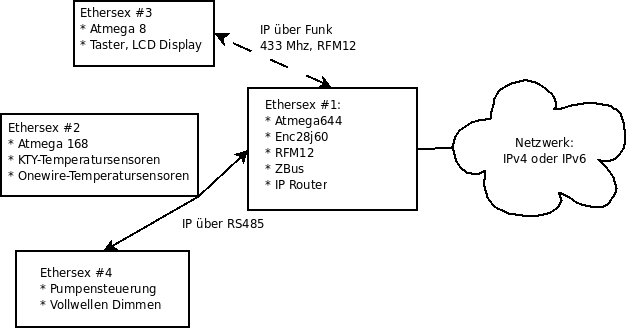
\includegraphics[width=8cm]{network-dia.png}
  \end{center}

\end{frame}


\section{Modulübersicht}
% \subsubsection{Netzwerk-anbindung}
\frame{
\frametitle{Ethersex features}
\begin{block}{Netzwerkanbindung}
\begin{itemize}
  \item Ethernet (ENC28J60) inkl. IEEE 802.1q (VLANs)
  \item USB (Software USB, Userland TUN Treiber)
  \item RFM12 (Funkübertragung auf dem 433 MHz ISM-Band)
  \item ZBus - Eigenes Protokoll für serielle Schnittstelle
\end{itemize}
\end{block}
}

% \subsubsection{Interaktion mit dem Anwender}
%% \frame{
%% \frametitle{Ethersex features}
%% \begin{block}{Interaktion mit dem Anwender}
%% \begin{itemize}
%%   \item HTTP-Server (mit Zugriff auf Dateien und ECMD)
%%   \item text-basiert (Telnet-ähnlich, TCP/IP oder UDP/IP)
%%   \item über serielle Schnittstelle
%%   \item über I2C
%%   \item via Jabber/XMPP
%%   \item via IRC
%% \end{itemize}
%% \end{block}
%% }

% \subsubsection{Netzwerkprotokolle}
\frame{
\frametitle{Ethersex features}
\begin{block}{Netzwerkprotokolle}
\begin{itemize}
  \item TCP/IP, UDP/IP und ICMP
  \item BOOTP (einfacherer, besser geeigneterer, Vorgänger von DHCP, der jedoch von allen gängigen DHCP-Servern unterstützt wird)
  \item TFTP (Upload von Firmwaredateien bzw. in den Data Flash Baustein)
  \item SYSLOG
  \item SNMP
  \item SMTP (E-Mail-Versand)
  \item NTP (Client und Server)
  \item DNS
\end{itemize}
\end{block}
}
\frame{
\frametitle{Ethersex features}
\begin{block}{Netzwerkprotokolle}
\begin{itemize}
  \item mDNS (Avahi)
  \item DynDNS
  \item MySQL (Client)
  \item IRC (Client)
  \item MPD (Music Player Daemon; einfache Steuerungsaufgaben)
  \item SOAP/XMLRPC
  \item UPnP
\end{itemize}
\end{block}
}

% \subsubsection{Kontakt zur Außenwelt}
% \frame[allowframebreaks]{
\frame{
\frametitle{Ethersex features}
\begin{block}{Kontakt zur Außenwelt}
\begin{itemize}
  \item RS232 und RS485
  \item Infrarotsender und -empfänger (RC5 Fernbedienungen!)
  \item I2C (Master und Slave)
  \item Steuerung von FS20-Modulen (Funkmodule von ELV bzw. Conrad, u.a. Steckdosen, Dimmer und Temperatursensoren)
  \item Modbus
  \item YPort (Serial over LAN (SOL) auch als XPort bekannt)
  \item Blinkenlights MCUF
  \item Porterweiterungen durch HC595 und HC165 möglich
\end{itemize}
\end{block}
}
\frame{
\frametitle{Ethersex features}
\begin{block}{Kontakt zur Außenwelt}
\begin{itemize}
  \item Dateneingabe mittels PS/2 Tastatur
  \item Dallas 1-wire Bus
  \item LCD (HD44780 und Kompatible)
  \item Philips dc3840 camera und MCA25-Handycam
  \item Stella Light (PWM für bis zu 8 Kanäle)
  \item Senertec Dachs MSR1 auslesen
  \item SMS
\end{itemize}
\end{block}
}

% \subsubsection{Verschiedenes}
\frame{
\frametitle{Ethersex features}
\begin{block}{Verschiedenes}
\begin{itemize}
  \item Fernsteuern von vielen Funksteckdosen mit RFM12 ASK
  \item Atmel DataFlash (SPI Flash)
  \item MMC/SD-Kartenleser
  \item Sound
  \item PAM Schicht zur Authentifizierung (z.b. ECMD-TCP)
  \item Systemuhr
  \item CRON-Dienst (analog dem crond auf Unix-Systemen)
  \item Pins können mit symbolischen Namen versehen werden
\end{itemize}
\end{block}
}
\frame{
\frametitle{Ethersex features}
\begin{block}{Verschiedenes}
\begin{itemize}
  \item Control6
  \item AliasCmd/Alias Namen für Befehle
  \item ECMD Scripting
  \item Virtuelles Dateisystem für DataFlash, MMC/SD-Karten und EEPROMs
  \item Netstat/Online Statistik
\end{itemize}
\end{block}
}




%% \subsection{Unterstütze Hardware}
%% \frame{
%%   \frametitle{Unterstütze Hardware}
%%   \begin{block}{Bausätze}
%%     \begin{itemize}
%%       \item Etherrape (fd0;lochraster.org)
%%       \item Net-IO (Pollin)
%%       \item AVR-Webserver (U. Radig)
%%       \item Thermotronic Basic (Eurotronic) \\Thermy (Aldi)
%%       \item ProBot (Conrad)
%%     \end{itemize}
%%   \end{block}
%% }

\section{Anwendungsfall}
\begin{frame}
  \frametitle{Anwendungsfall}
  
  
  \begin{block}{Voraussetzungen}
    \begin{itemize}
    \item Ziel: Blockheizkraftwerk (5.5kW) ans Netz anschließen
    \item BHKW schreibt alle 10s auf serieller Schnittstelle Betriebsdaten
    \end{itemize}
  \end{block}

  
  \begin{block}{Daten auffangen}
    \begin{itemize}
    \item Neues Modulerstellen
    \item Usart im Menuconfig anfordern
    \item Im Receive Interrupthandler werden Daten in Buffer geschrieben
    \item Periodisch aufgerufene Funktion prüft Checksumme
    \end{itemize}
  \end{block}

\end{frame}


\begin{frame}
  \frametitle{Anwendungsfall}
  
  \begin{block}{Daten bereitstellen}
    \begin{itemize}
    \item Neues ECMD definieren (bsp. \t{msr1 get})
    \item ECMD liefert validen Buffer zurück
    \item Daten sind nun beispielsweise per HTTP verfügbar
    \end{itemize}
  \end{block}

  
  \begin{block}{Visualisieren}
    \begin{itemize}
    \item Statische HTML Seite im internen Flash mit JS
    \item Javascript holt per XMLReqest ECMD Daten ab
    \item \t{GET 1.1 /ecmd?msr1+get}
    \item JS frickelt Daten in HTML Seite
    \end{itemize}
  \end{block}
\end{frame}


\begin{frame}
  \begin{center}
    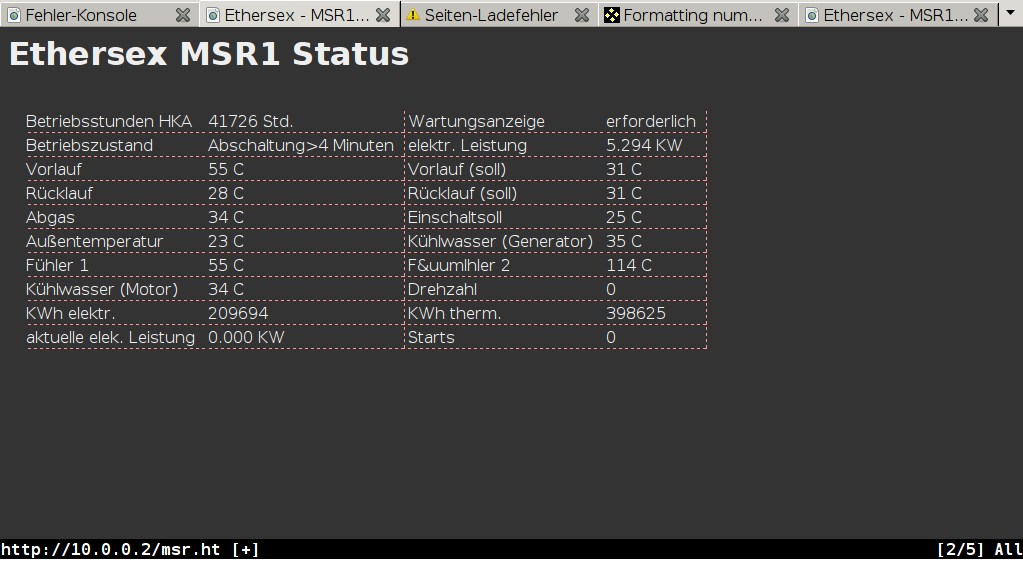
\includegraphics[width=11.1cm]{Msr1_screenshot.png}
  \end{center}
\end{frame}

\begin{frame}
  
  \begin{itemize}
  \item Client Side Javascript innerhalb von SVG
  \end{itemize}

    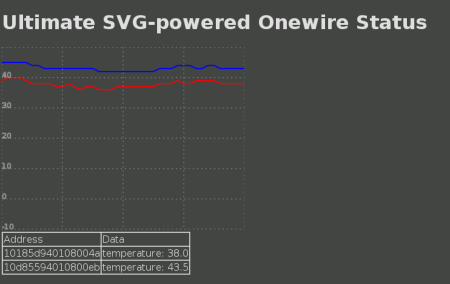
\includegraphics[width=6cm]{Onewire-svg.png}

\end{frame}


\begin{frame}
  \frametitle{Anwendungsfall}
  
  \begin{block}{Ein bischen Steuerung}
    \begin{itemize}
    \item Control6 Skript ließt Betriebsdaten aus (Temperatur, ...)
    \item C6: Speichert die Daten selbständig auf SD Karte
    \item C6: Sendet Syslognachricht, bei zu hoher Temperatur
    \item Cron Daemon schaltet BHKW passend zum Frühstück an
    \end{itemize}
  \end{block}

\end{frame}

\section{Projekte}
\begin{frame}
  \frametitle{entstandene Projekte}

  \begin{itemize}
  \item div. Heizungssteuerungen, Temperaturerfassung, ...
  \item Solaranlagen-, BHKW-Überwachung, ...
  \item Biogas-Anlage
  \item volkszaehler.org
  \item Nistkastenüberwachung
  \item matemat @Kapsel
  \end{itemize}

\end{frame}

\section{Mitmachen \& Fragen}
\begin{frame}
  \frametitle{Mitmachen}
  \begin{itemize}
  \item Workshop im Anschluss
  \item Wiki: http://ethersex.de
  \item Mailingliste: ethersex-devel@list.zerties.org
  \item IRC:  \#ethersex in freenode
  \item fork us @ github
  \end{itemize}

\end{frame}

\frame{
\frametitle{www.ethersex.de}
Fragen? \\
Anregungen? \\
\bigskip 
\bigskip 
\bigskip 
\begin{center}
\textbf{Danke für die Aufmerksamkeit!}\end{center}
\bigskip 
\bigskip 
\bigskip 
\begin{center}
 \begin{small}Projekt-Wiki: \texttt{www.ethersex.de} \end{small}
\end{center}
}
\end{document}
